% Options for packages loaded elsewhere
\PassOptionsToPackage{unicode}{hyperref}
\PassOptionsToPackage{hyphens}{url}
\PassOptionsToPackage{dvipsnames,svgnames,x11names}{xcolor}
%
\documentclass[
  10pt,
  titlepage=firstiscover,
  toc=flat,
  twoside]{scrreprt}

\usepackage{amsmath,amssymb}
\usepackage{iftex}
\ifPDFTeX
  \usepackage[T1]{fontenc}
  \usepackage[utf8]{inputenc}
  \usepackage{textcomp} % provide euro and other symbols
\else % if luatex or xetex
  \usepackage{unicode-math}
  \defaultfontfeatures{Scale=MatchLowercase}
  \defaultfontfeatures[\rmfamily]{Ligatures=TeX,Scale=1}
\fi
\usepackage{lmodern}
\ifPDFTeX\else  
    % xetex/luatex font selection
    \setmainfont[]{Montserrat}
    \setsansfont[]{Old Newspaper Font}
    \setmonofont[]{cascadia-code}
\fi
% Use upquote if available, for straight quotes in verbatim environments
\IfFileExists{upquote.sty}{\usepackage{upquote}}{}
\IfFileExists{microtype.sty}{% use microtype if available
  \usepackage[]{microtype}
  \UseMicrotypeSet[protrusion]{basicmath} % disable protrusion for tt fonts
}{}
\makeatletter
\@ifundefined{KOMAClassName}{% if non-KOMA class
  \IfFileExists{parskip.sty}{%
    \usepackage{parskip}
  }{% else
    \setlength{\parindent}{0pt}
    \setlength{\parskip}{6pt plus 2pt minus 1pt}}
}{% if KOMA class
  \KOMAoptions{parskip=half}}
\makeatother
\usepackage{xcolor}
\setlength{\emergencystretch}{3em} % prevent overfull lines
\setcounter{secnumdepth}{-\maxdimen} % remove section numbering
% Make \paragraph and \subparagraph free-standing
\makeatletter
\ifx\paragraph\undefined\else
  \let\oldparagraph\paragraph
  \renewcommand{\paragraph}{
    \@ifstar
      \xxxParagraphStar
      \xxxParagraphNoStar
  }
  \newcommand{\xxxParagraphStar}[1]{\oldparagraph*{#1}\mbox{}}
  \newcommand{\xxxParagraphNoStar}[1]{\oldparagraph{#1}\mbox{}}
\fi
\ifx\subparagraph\undefined\else
  \let\oldsubparagraph\subparagraph
  \renewcommand{\subparagraph}{
    \@ifstar
      \xxxSubParagraphStar
      \xxxSubParagraphNoStar
  }
  \newcommand{\xxxSubParagraphStar}[1]{\oldsubparagraph*{#1}\mbox{}}
  \newcommand{\xxxSubParagraphNoStar}[1]{\oldsubparagraph{#1}\mbox{}}
\fi
\makeatother


\providecommand{\tightlist}{%
  \setlength{\itemsep}{0pt}\setlength{\parskip}{0pt}}\usepackage{longtable,booktabs,array}
\usepackage{calc} % for calculating minipage widths
% Correct order of tables after \paragraph or \subparagraph
\usepackage{etoolbox}
\makeatletter
\patchcmd\longtable{\par}{\if@noskipsec\mbox{}\fi\par}{}{}
\makeatother
% Allow footnotes in longtable head/foot
\IfFileExists{footnotehyper.sty}{\usepackage{footnotehyper}}{\usepackage{footnote}}
\makesavenoteenv{longtable}
\usepackage{graphicx}
\makeatletter
\def\maxwidth{\ifdim\Gin@nat@width>\linewidth\linewidth\else\Gin@nat@width\fi}
\def\maxheight{\ifdim\Gin@nat@height>\textheight\textheight\else\Gin@nat@height\fi}
\makeatother
% Scale images if necessary, so that they will not overflow the page
% margins by default, and it is still possible to overwrite the defaults
% using explicit options in \includegraphics[width, height, ...]{}
\setkeys{Gin}{width=\maxwidth,height=\maxheight,keepaspectratio}
% Set default figure placement to htbp
\makeatletter
\def\fps@figure{htbp}
\makeatother

\usepackage{multicol}
\makeatletter
\@ifpackageloaded{caption}{}{\usepackage{caption}}
\AtBeginDocument{%
\ifdefined\contentsname
  \renewcommand*\contentsname{Table of contents}
\else
  \newcommand\contentsname{Table of contents}
\fi
\ifdefined\listfigurename
  \renewcommand*\listfigurename{List of Figures}
\else
  \newcommand\listfigurename{List of Figures}
\fi
\ifdefined\listtablename
  \renewcommand*\listtablename{List of Tables}
\else
  \newcommand\listtablename{List of Tables}
\fi
\ifdefined\figurename
  \renewcommand*\figurename{Figure}
\else
  \newcommand\figurename{Figure}
\fi
\ifdefined\tablename
  \renewcommand*\tablename{Table}
\else
  \newcommand\tablename{Table}
\fi
}
\@ifpackageloaded{float}{}{\usepackage{float}}
\floatstyle{ruled}
\@ifundefined{c@chapter}{\newfloat{codelisting}{h}{lop}}{\newfloat{codelisting}{h}{lop}[chapter]}
\floatname{codelisting}{Listing}
\newcommand*\listoflistings{\listof{codelisting}{List of Listings}}
\makeatother
\makeatletter
\makeatother
\makeatletter
\@ifpackageloaded{caption}{}{\usepackage{caption}}
\@ifpackageloaded{subcaption}{}{\usepackage{subcaption}}
\makeatother

\ifLuaTeX
\usepackage[bidi=basic]{babel}
\else
\usepackage[bidi=default]{babel}
\fi
\babelprovide[main,import]{english}
\ifPDFTeX
\else
\babelfont{rm}[]{Montserrat}
\fi
% get rid of language-specific shorthands (see #6817):
\let\LanguageShortHands\languageshorthands
\def\languageshorthands#1{}
\ifLuaTeX
  \usepackage{selnolig}  % disable illegal ligatures
\fi
\usepackage{bookmark}

\IfFileExists{xurl.sty}{\usepackage{xurl}}{} % add URL line breaks if available
\urlstyle{same} % disable monospaced font for URLs
\hypersetup{
  pdftitle={Shadowdark Template},
  pdfauthor={John Doe},
  pdflang={en},
  colorlinks=true,
  linkcolor={blue},
  filecolor={Maroon},
  citecolor={Blue},
  urlcolor={black},
  pdfcreator={LaTeX via pandoc}}

% ------------------------------------------------------------------------------------- %
%                                        PACKAGES                                       %
% ------------------------------------------------------------------------------------- %
\usepackage[onehalfspacing]{setspace}
\usepackage{etoolbox}
\usepackage[most]{tcolorbox}
\tcbset{beforeafter skip balanced = 0.5\baselineskip plus 2pt}
\usepackage{calc}
\usepackage{xparse}
\usepackage{tikz}
\usetikzlibrary{positioning,calc}
\usepackage{tikzpagenodes}
\usepackage{enumitem}
\usepackage[explicit]{titlesec}
\usepackage{eso-pic}
\usepackage{multicol}
\usepackage[toc]{multitoc}
\usepackage{dblfloatfix}
\usepackage{scrlayer-scrpage}
\usepackage{wrapfig}
\usepackage{tabularray}

% ------------------------------------------------------------------------------------- %
%                                        GEOMETRY                                       %
% ------------------------------------------------------------------------------------- %
\newlength{\sdBleed}
\newlength{\sdLeftAdjust}
\newlength{\sdRightAdjust}
\newlength{\sdTop}
\newlength{\sdBottom}
\newlength{\sdLeft}
\newlength{\sdRight}
\setlength\sdBleed{0cm}
\setlength\sdLeftAdjust{0cm/2}
\setlength\sdRightAdjust{0cm/2}
\setlength\sdTop{1.25cm+\sdBleed}
\setlength\sdBottom{1.5cm+\sdBleed}
\setlength\sdLeft{1cm+\sdLeftAdjust}
\setlength\sdRight{1cm+\sdRightAdjust}
\usepackage[%
  paperwidth=14.8cm+\sdBleed,
  paperheight=21cm+\sdBleed+\sdBleed,
  top=\sdTop,
  bottom=\sdBottom,
  left=\sdLeft,
  right=\sdRight
]{geometry}

% ------------------------------------------------------------------------------------- %
%                                         BASICS                                        %
% ------------------------------------------------------------------------------------- %
% ------------------------------------ Text Layout ------------------------------------ %

% --------------------------------------- Fonts --------------------------------------- %
\newfontfamily{\displayfont}{JSL Blackletter}

\usepackage{lettrine}
\renewcommand\LettrineFontHook{\displayfont}

% -------------------------------------- Spacing -------------------------------------- %
\setlength{\columnsep}{20pt}
\setlength{\intextsep}{0pt}

% --------------------------------------- Lists --------------------------------------- %
\setlist[description]{
  font=\normalfont\bfseries,
}
\renewcommand{\labelitemi}{$\bullet$}
\renewcommand{\labelitemii}{\textbullet}
\renewcommand{\labelitemiii}{\textbullet}

% ------------------------------------ Toc Entries ------------------------------------ %
\setkomafont{partentry}{\normalfont\large\bfseries}
\setkomafont{chapterentry}{\normalfont\bfseries}

% ------------------------------------- No Labels ------------------------------------- %
\renewcommand*{\figureformat}{}
\renewcommand*{\tableformat}{}
\renewcommand*{\captionformat}{}

% ------------------------------------ Table Rules ------------------------------------ %
\renewcommand{\toprule}[2]{}
\renewcommand{\bottomrule}[2]{}

% --------------------------------------- Footer -------------------------------------- %
\clearscrheadfoot
\ofoot*{%
  \ifthispageodd{%
    \begin{tikzpicture}[overlay,remember picture]
      \node[black] at ($(current page text area.south east)+(0,-0.8)$) {\pagemark};
    \end{tikzpicture}%
  }{%
    \begin{tikzpicture}[overlay,remember picture]
      \node[black] at ($(current page text area.south west)+(0.15,-0.8)$) {\pagemark};
    \end{tikzpicture}%
  }
}


% ------------------------------------------------------------------------------------- %
%                                       SECTIONING                                      %
% ------------------------------------------------------------------------------------- %
\titleclass{\part}{top}
\titlespacing*{\part}{0pt}{0cm}{0pt}
\titleformat{\part}[block]%
  {\fontsize{46}{30}\selectfont\displayfont}%format
  {}%label
  {0pt}%sep
  {%
    \vspace{-1cm}
    \begin{center}
    #1
  }%before
  [{%
    \vspace{-6mm}
    \includegraphics[width=\linewidth]{\_extensions/shadowdark/assets/ShadowDark\_Page-Art\_Line\_A.png}
    \end{center}
  }]%after

\titleformat{\chapter}[block]
{}
{}%label
{0pt}%sep
{\begin{tikzpicture}[overlay,remember picture]
  \fill[black] (current page.north west) rectangle ($(current page.north east)+(0,-3)-(0,\sdBleed)$);
  \node[white] at ($(current page.north)+(0,-1.5)-(0,\sdBleed)$) {\fontsize{33}{30} \selectfont\sffamily{#1}};
\end{tikzpicture}}
[]%after
\titlespacing*{\chapter}{0pt}{0pt}{4mm}

\titleformat{\section}[block]%
  {\Large\bfseries}%format
  {}%label
  {0pt}%sep
  {#1}%before
  [{\titlerule[1pt]}]%after
\titlespacing*{\section}{0pt}{0pt}{0pt}

\titleformat{\subsection}[display]%
{}%format
{}%label
{0pt}%sep
{\colorbox{black}{\parbox{\dimexpr\columnwidth}{\vspace{4pt}\centering\Large\normalfont\bfseries\color{white}#1\vspace{4pt}}}}
[]%after
\titlespacing*{\subsection}{0pt}{2pt}{-2pt}

\titleformat{\subsubsection}[display]%
{\Large\bfseries}%format
{}%label
{0pt}%sep
{#1}%before
[]%after
\titlespacing*{\subsubsection}{0pt}{0pt}{-4pt}

\titleformat{\paragraph}[display]%
{}%format
{}%label
{0pt}%sep
{\colorbox{black}{\parbox{\dimexpr\columnwidth}{\vspace{4pt}\centering\Large\normalfont\bfseries\color{white}#1\vspace{4pt}}}}
[]%after
\titlespacing*{\paragraph}{0pt}{2pt}{-8pt}

\titleformat{\subparagraph}[runin]%
{\large\bfseries}%format
{}%label
{0pt}%sep
{#1}%before
[{\:}]%after
\titlespacing*{\subparagraph}{0pt}{0pt}{0pt}

% ------------------------------------------------------------------------------------- %
%                                         TITLE                                         %
% ------------------------------------------------------------------------------------- %

% ---------------------------------- Titlepage Macro ---------------------------------- %
\newcommand{\shadowdarkTitlePage}{%
  \clearpage
  \thispagestyle{empty}
  \AddToShipoutPictureBG*{\put(0.3cm+\sdLeftAdjust,2cm+\sdBleed){\includegraphics[height=17cm]{\_extensions/shadowdark/assets/ShadowDark\_Page-Art\_Tree\_01.png}}}
  \AddToShipoutPictureBG*{\put(\pagewidth - 3cm - \sdRightAdjust,2cm+\sdBleed){\includegraphics[height=17cm]{\_extensions/shadowdark/assets/ShadowDark\_Page-Art\_Tree\_02.png}}}

  \newgeometry{left=21mm+\sdLeft,right=22mm+\sdRight, top=2.5cm+\sdBleed, bottom=1.25cm+\sdBleed}

  \begin{center}

    \resizebox{\textwidth}{!}{\displayfont{Shadowdark Template}}
    
  \vspace{-1mm}
  \includegraphics[width=\textwidth]{\_extensions/shadowdark/assets/ShadowDark\_Page-Art\_Line\_A.png}

    \vspace{-5mm}
  \sffamily\large{A template for Shadowdark RPG}
  \vspace{-2mm}
    \end{center}

    \footnotesize\textbf{Writing, Design, Layout}
  \vspace{3pt}
  \hrule
  \vspace{-3pt}

  \scriptsize
  John Doe
  
    \footnotesize\textbf{Art}
  \vspace{3pt}
  \hrule
  \vspace{-3pt}

  \scriptsize
  This work includes artwork from
  \url{https://arcanum-rpg-studio.itch.io/rt-assets-shadowdark}. The
  artwork is licensed under the Creative Commons Attribution 4.0
  International License available at
  \url{https://creativecommons.org/licenses/by/4.0/legalcode}.
  
    \footnotesize\textbf{Fonts}
  \vspace{3pt}
  \hrule
  \vspace{-3pt}

  \scriptsize
  JSL Blackletter font © 2023 Jeffrey S. Lee.\\
  Old Newspaper Types font © 2023 Manfred Klein.\\
  Montserrat font family © 2023 Julieta Ulanovsky, Sol Matas, Juan Pablo
  del Peral, Jacques Le Bailly.
  
    \footnotesize\textbf{Legal Information and Attribution Statement}
  \vspace{3pt}
  \hrule
  \vspace{-3pt}
  
  \scriptsize
      This work is an independent product published under the Shadowdark
      RPG Third-Party License and is not affiliated with The Arcane
      Library, LLC. Shadowdark RPG © 2023 The Arcane Library, LLC.
  
      This work is licensed under the Creative Commons Attribution 4.0
      International License. This work uses material licensed by the
      Shadowdark RPG Third-Party License, and that material is not
      included in this license. To view a copy of this license, visit
      \url{http://creativecommons.org/licenses/by/4.0/} or send a letter
      to Creative Commons, PO Box 1866, Mountain View, CA 94042, USA.
  
  \begin{center}
  \vfill
  \includegraphics[width=5cm]{\_extensions/shadowdark/assets/Third Party
Shadowdark Logo Black.png}
  \end{center}
  \clearpage
  \restoregeometry
  \normalsize
}

% --------------------------------- Titlepage is Cover -------------------------------- %
\newcommand{\shadowdarkTitlePageAsCover}{%
  \clearpage
  \thispagestyle{empty}
  \begin{center}
  \vspace*{1cm}
  \color{black}%
  \fontsize{46}{30}\selectfont\displayfont{Shadowdark Template}

  \vspace{-6mm}
  \includegraphics[width=\linewidth]{\_extensions/shadowdark/assets/ShadowDark\_Page-Art\_Line\_A.png}
  
  \vspace{-5mm}
    \sffamily\normalsize\bfseries{A template for Shadowdark RPG}
  
    \vspace{-4mm}
    
    \sffamily\LARGE\bfseries{John Doe}
  
  \includegraphics{\_extensions/shadowdark/assets/ShadowDark\_Page-Art\_Triangle\_01.png}

  \vfill
  \includegraphics[width=8cm]{\_extensions/shadowdark/assets/Third Party
Shadowdark Logo Black.png}
  \end{center}

  \clearpage
  \normalsize
}

% -------------------------------------- Backside ------------------------------------- %
\newcommand{\makecoverback}{%
  \clearpage
  \addtocounter{page}{-1}
  \thispagestyle{empty}
  \begin{center}
          \small{\phantom{image}\AddToShipoutPictureBG*{\includegraphics[width=\paperwidth, height=\paperheight]{assets/images/map.png}}}
          \end{center}
}

\newcommand{\makebastardtitle}{%
  \clearpage
  \addtocounter{page}{-1}
  \thispagestyle{empty}
  \Large{Shadowdark Template}
  
    \large{John Doe}
    \clearpage
  \addtocounter{page}{-1}
  \thispagestyle{empty}
  \phantom{bastardback}
}

\newcommand{\makelegalback}{%
  \clearpage
  \thispagestyle{empty}
  \begin{center}
      \small{This work is an independent product published under the
Shadowdark RPG Third-Party License and is not affiliated with The Arcane
Library, LLC. Shadowdark RPG © 2023 The Arcane Library, LLC.}
  
        \small{This work includes artwork from
\url{https://arcanum-rpg-studio.itch.io/rt-assets-shadowdark}. The
artwork is licensed under the Creative Commons Attribution 4.0
International License available at
\url{https://creativecommons.org/licenses/by/4.0/legalcode}.}
  
        \small{JSL Blackletter font © 2023 Jeffrey S. Lee.\\
Old Newspaper Types font © 2023 Manfred Klein.\\
Montserrat font family © 2023 Julieta Ulanovsky, Sol Matas, Juan Pablo
del Peral, Jacques Le Bailly.}
  
      \phantom{Copyright}
    \vfill
    \small{This work is licensed under the Creative Commons Attribution
4.0 International License. This work uses material licensed by the
Shadowdark RPG Third-Party License, and that material is not included in
this license. To view a copy of this license, visit
\url{http://creativecommons.org/licenses/by/4.0/} or send a letter to
Creative Commons, PO Box 1866, Mountain View, CA 94042, USA.}
    \end{center}
}

\newcommand{\maketitlepageback}{%
  \clearpage
  \thispagestyle{empty}
  \begin{center}
      \end{center}
}

% ------------------------------------- Maketitle ------------------------------------- %
\NewCommandCopy{\oldmaketitle}{\maketitle}
\renewcommand{\maketitle}{%
      \phantom{cover}\AddToShipoutPictureFG*{\includegraphics[width=\paperwidth, height=\paperheight, keepaspectratio=false]{assets/images/template\_cover.png}}
    \addtocounter{page}{-1}
    \thispagestyle{empty}

          \makecoverback
      
  
            \shadowdarkTitlePage
          }
\title{Shadowdark Template}
\usepackage{etoolbox}
\makeatletter
\providecommand{\subtitle}[1]{% add subtitle to \maketitle
  \apptocmd{\@title}{\par {\large #1 \par}}{}{}
}
\makeatother
\subtitle{A template for Shadowdark RPG}
\author{John Doe}
\date{}

\begin{document}
\maketitle

\renewcommand*\contentsname{Table of contents}
{
\hypersetup{linkcolor=}
\setcounter{tocdepth}{2}
\tableofcontents
}

\part{Part 1}

\begin{center}

\vspace{-5mm}

\vspace{-3mm}

\sffamily\normalsize\bfseries{A part can have a subtitle}


\includegraphics{_extensions/shadowdark/assets/ShadowDark_Page-Art_Triangle_01.png}

\vfill

\begin{tikzpicture}[overlay,remember picture]

\node[black] at ($(current page.south)+(0,4)$) {
\includegraphics{_extensions/shadowdark/assets/ShadowDark_Page-Art_Header_02.png}};

\node[white] at ($(current page.south)+(0.2,4.1)$) {\parbox{8.5cm}{\centering\large\sffamily{And a banner with some text}}};

\end{tikzpicture}

\end{center}

\chapter{Basics}\label{basics}

{\begin{multicols}{2}

\lettrine[lines=3]{D}{rop caps} can be done like this. You can give them
an option attribute, if you need special commands. See the lettrine
latex package.

\subsubsection{Global options}\label{global-options}

You can customize the template through the frontmatter.

If you set \texttt{justified:\ false}, the document is now ragged.

With the cover variable you can set an image to be used as the cover.
You can also add images or text to the backside of it through the
frontmatter.

For the title page you have three options:

\begin{enumerate}
\def\labelenumi{\arabic{enumi}.}
\tightlist
\item
  Like in this template. This is the default. The title font size is set
  automatically. If this doesn't look good, you can set it with
  \texttt{title-font-size:\ number}.
\item
  With \texttt{title-is-cover:\ true} the titlepage is styled more like
  a part and can function as a cover.
\item
  If you don't need a titlepage, use \texttt{no-title-page:\ true}
\end{enumerate}

\subsubsection{Two column mode}\label{two-column-mode}

You can wrap text inside a two column section. There are some
limitations with this

\begin{itemize}
\tightlist
\item
  You need to exclude level 1 headings from these
\item
  Table support is very limited (see below)
\end{itemize}

You can however easily switch between one and two columns.

Columns can have a \texttt{ragged} class, which allows them to be
uneven. The \texttt{unbalanced} class is similar, but has its drawbacks.
You can try it, if ragged isn't sufficient.

Inside two column mode, prefer to use either level 4 headings or level 3
headings, like in the Shadowdark book.

\subsubsection{Heading 4}\label{heading-4}

These are the normal headings in two column mode.

\subsubsection{A simple Table}\label{a-simple-table}

Inside two columns mode, only very simple tables are supported and need
special syntax. For table headings use level 5 headings.

\paragraph{TABLE}\label{table}

\begin{center}

\begin{tblr}{cc}

\textbf{d6} &\textbf{Effect} \\

\hline

1 &nostrud \\

2 &ipsum \\

3 &fugiat \\

4 &irure \\

5 &labore \\

6 &nulla \\

\end{tblr}

\end{center}

\subsubsection{Images}\label{images}

This template has some utility functions for images. Just give an image
the class you want to use.

These options are available:

\textbf{fullpage:} Starts a new page and fills it with the image. If you
give the \texttt{.stretch} class also, it ignores the aspect ratio to
fill the space completly.

\textbf{fullpage-bg:} Similar to above, but doesn't start a new page and
inserts the image as the background of the current page.

\textbf{wrap:} Wrap text around the image. Accepts two attributes.
\texttt{position} can be ``l'', ``r'' or ``c'' and determines where the
image is inserted. Defaults to ``l''. \texttt{wx} is a number between 0
and 1 and describes the percentile width of the image.

\textbf{fill:} Inserts the image in float mode. Places it where it fits
as is.

\textbf{wide:} As fill, but the image has the width of the text.

\textbf{bottom:} Place the image directly at the bottom margin.

\textbf{bottom-left:} Place the image at the bottom left cólumn.

\textbf{bottom-right:} Place the image at the bottom right cólumn.

\textbf{place:} Place the image by hand.

\AddToShipoutPictureFG*{\AtPageLowerLeft{\put(\sdLeft,\sdBottom){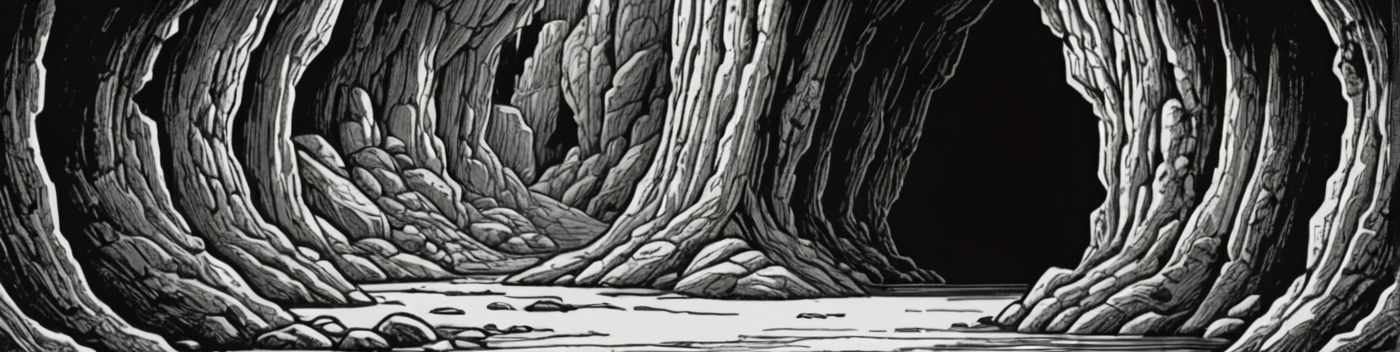
\includegraphics[width=\textwidth]{assets/images/cave_small.png}}}}

\end{multicols}
}

\chapter{Monster Statistics}\label{monster-statistics}

{\begin{multicols}{2}

\subsection{Header 3}\label{header-3}

You can use a json file with monster stats and headers with the monster
class to show them. You could also give the monster stats directly as
json in a codeblock. This supports images, if they are given in the
json. Of course you can also just format them yourself.

\subsection{BANDIT}\label{bandit}

\emph{Hard-bitten rogue in tattered leathers and a hooded cloak.}

\textbf{AC} 13, \textbf{HP} 4, \textbf{ATK} 1 club +1 (1d4) or 1 shortbow (far) +0 (1d4), \textbf{MV} near, \textbf{S} +1, \textbf{D} +0, \textbf{C} +0, \textbf{I} -1, \textbf{W} +0, \textbf{Ch} -1, \textbf{AL} C, \textbf{LV} 1

\textbf{Ambush. }Deal an extra die of damage when undetected.

\subsection{BLACK PUDDING}\label{black-pudding}

\emph{A black, ice-cold mass of sludge.}

\textbf{AC} 9, \textbf{HP} 30, \textbf{ATK} 3 tentacle +4 (2d6), \textbf{MV} near (climb), \textbf{S} +2, \textbf{D} -1, \textbf{C} +3, \textbf{I} -4, \textbf{W} -3, \textbf{Ch} -4, \textbf{AL} N, \textbf{LV} 6

\textbf{Impervious. }Only damaged by fire.\\
\textbf{Corrosive.
}Wood or metal that touches the ooze dissolves on a d6 roll of 1-3.

\end{multicols}
}

\section{Short Monster stats}\label{short-monster-stats}

If you want to include short statblocks, for example in adventures, you
can do it like this.

{\raggedcolumns\begin{multicols}{2}

\textbf{Ape}

\textbf{AC} 12, \textbf{HP} 10, \textbf{ATK} 1 fist +2 (1d6) or 1 rock (far) +2 (1d4), \textbf{MV} near (climb), \textbf{S} 2, \textbf{D} 2, \textbf{C} 1, \textbf{I} -2, \textbf{W} 1, \textbf{Ch} 0, \textbf{AL} N, \textbf{LV} 2\\

\columnbreak

\textbf{Bandit}

\textbf{AC} 13, \textbf{HP} 4, \textbf{ATK} 1 club +1 (1d4) or 1 shortbow (far) +0 (1d4), \textbf{MV} near, \textbf{S} 1, \textbf{D} 0, \textbf{C} 0, \textbf{I} -1, \textbf{W} 0, \textbf{Ch} -1, \textbf{AL} C, \textbf{LV} 1\\
\textbf{Ambush. }Deal an extra die of damage when undetected.

\end{multicols}
}

\chapter{Spells}\label{spells}

{\begin{multicols*}{2}

Spells work similar to monsters.

\subsection{ALARM}\label{alarm}

\emph{Tier 1, wizard}

\textbf{Duration: }1 day

\textbf{Range: }Close

You touch one object, such as a door threshold, setting a magical alarm
on it. If any creature you do not designate while casting the spell
touches or crosses past the object, a magical bell sounds in your head.

\subsection{BURNING HANDS}\label{burning-hands}

\emph{Tier 1, wizard}

\textbf{Duration: }Instant

\textbf{Range: }Close

You spread your fingers with thumbs touching, unleashing a circle of
flame that roars out to a close area around where you stand.

Creatures within the area of effect take 1d6 damage, and flammable
objects catch fire.

\subsection{CREATE UNDEAD}\label{create-undead}

\emph{Tier 5, wizard}

\textbf{Duration: }1 day

\textbf{Range: }Close

You conjure a vengeful undead creature to do your bidding.

When you cast this spell, you choose to summon either a wight or wraith.
It appears next to you and is under your control.

The undead creature acts on your turn. After 1 day, it melts away into
smoke.

\AddToShipoutPictureFG*{\AtPageLowerLeft{\put(0cm+\columnwidth + \columnsep + \sdLeft,0cm + \sdBottom){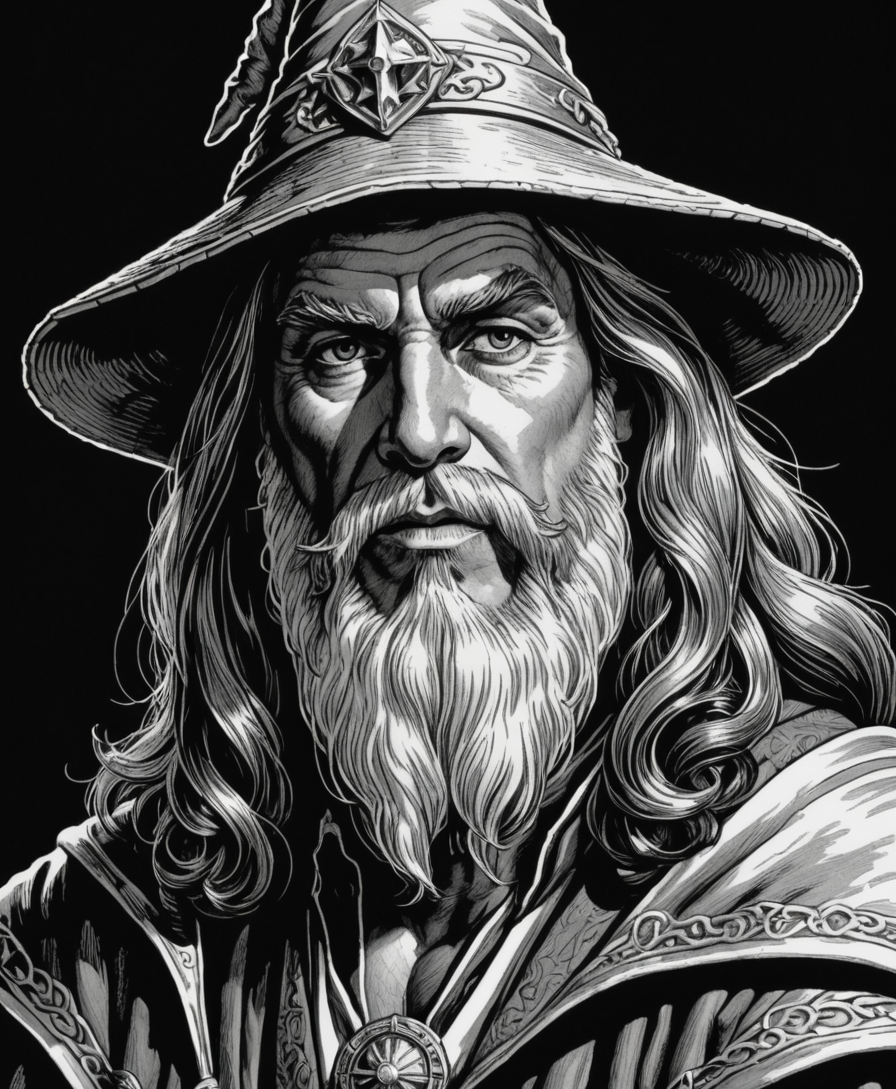
\includegraphics[width=\columnwidth]{assets/images/wizard.png}}}}

\end{multicols*}
}

\clearpage\phantom{image}\AddToShipoutPictureFG*{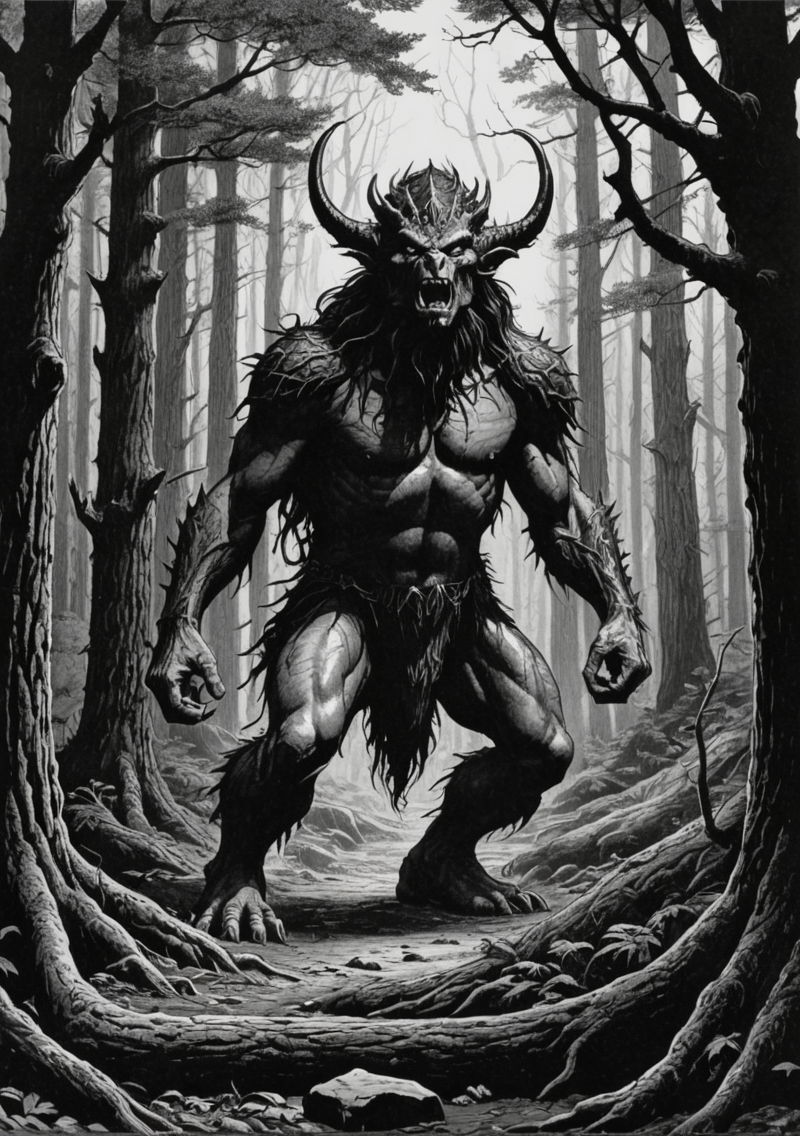
\includegraphics[keepaspectratio=false,width=\paperwidth, height=\paperheight]{assets/images/monster_page.png}}

\part{Adventures}

\begin{center}

\vspace{-5mm}

\vspace{-3mm}

\sffamily\normalsize\bfseries{A 1st-level adventure for Shadowdark RPG}


\includegraphics{_extensions/shadowdark/assets/ShadowDark_Page-Art_Triangle_01.png}

\vfill


\includegraphics{_extensions/shadowdark/assets/ShadowDark_Spot-Art_001.png}

\end{center}

\chapter{Overview}\label{overview}

\subsubsection{Header 4}\label{header-4}

Adventures use a single column.

\subsubsection{BACKGROUND}\label{background}

Adipisicing elit occaecat et ut aute. Adipisicing veniam anim nulla
fugiat aliquip duis ad. Do commodo eu consequat exercitation elit. Do do
amet consectetur do veniam in. Quis ad enim ullamco eiusmod exercitation
et id veniam enim aute ea et pariatur Lorem. Et eu ex eiusmod sint
cupidatat est.

Consequat anim ullamco velit voluptate labore. Incididunt cillum sunt
pariatur Lorem elit occaecat deserunt eu labore et quis labore
voluptate. Velit fugiat ea incididunt eu consectetur anim amet eu ex.
Officia commodo amet ipsum voluptate elit. Enim minim mollit dolor nisi
officia aliqua veniam laboris. Et dolore et reprehenderit sint esse
magna eu. Do adipisicing incididunt et veniam est laboris labore do
officia amet.

\subsubsection{FACTIONS}\label{factions}

\subparagraph{Consequat}\label{consequat}

Tempor enim exercitation ut veniam ex commodo amet do. Do ea dolore
nostrud proident culpa. Ea laboris veniam dolor do dolore eiusmod veniam
incididunt sint reprehenderit adipisicing. Et exercitation fugiat aute
eu et Lorem tempor esse qui.

\subparagraph{Mminim}\label{mminim}

Incididunt elit velit fugiat velit id adipisicing do pariatur laboris.
Sunt aute aliquip occaecat ipsum duis et. Consectetur laborum amet
officia fugiat. Elit tempor labore amet elit cillum est et ullamco. Do
sunt nisi ex minim magna nostrud Lorem aute laborum minim eiusmod. Ad
esse labore minim sunt esse occaecat voluptate duis amet sit aute dolore
do.

\subsubsection{Ullamco}\label{ullamco}

\vspace*{4pt}\begin{wrapfigure}{l}{0.28\textwidth}\centering\begin{tikzpicture}\clip (0,0) circle (0.14\textwidth);\path (0,0) node {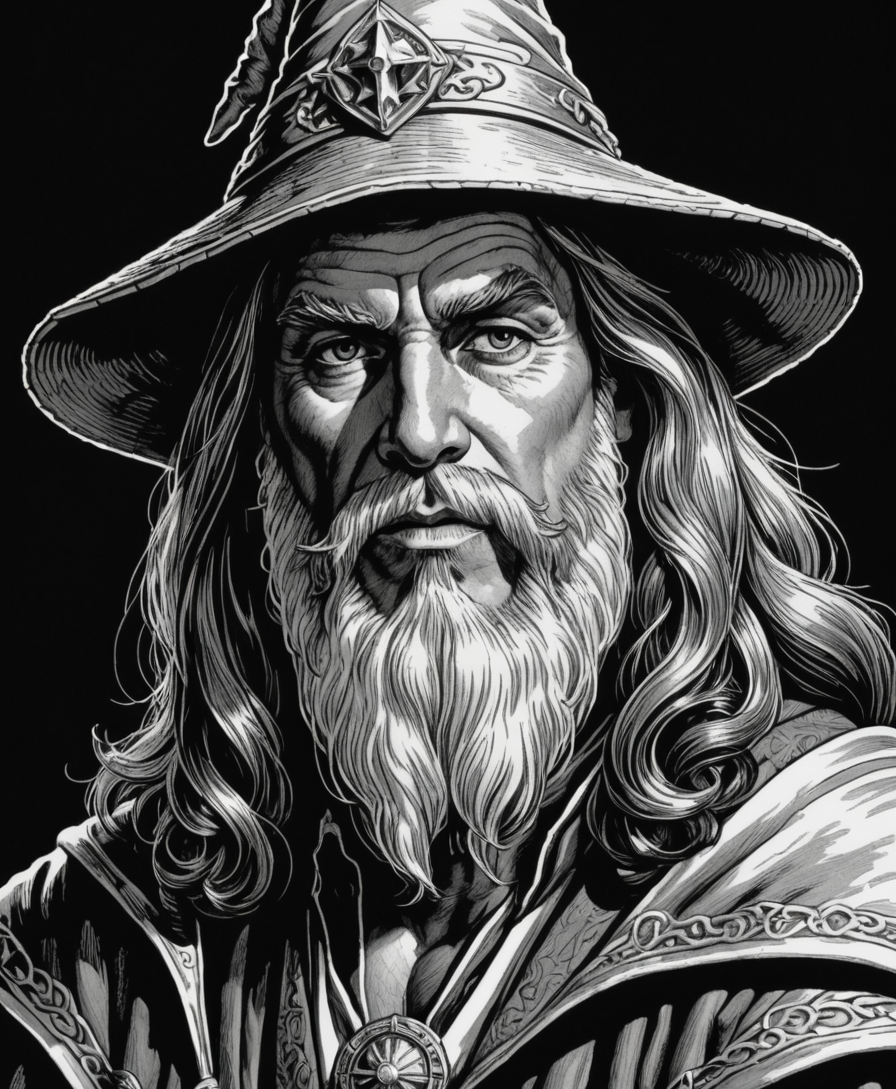
\includegraphics[width=0.28\textwidth]{assets/images/wizard.png}};\end{tikzpicture}\end{wrapfigure}

Consequat sint ipsum non non incididunt. Aute consectetur occaecat
ullamco incididunt voluptate consequat veniam ea. Sint esse consequat
duis do. Dolore adipisicing excepteur eiusmod quis laborum.

Ea cillum aliquip amet veniam tempor et culpa ipsum non. Eiusmod
adipisicing eu reprehenderit eu ut sunt eu. Do sunt fugiat laboris irure
ut. Laborum eu non minim sunt sit.

\subsubsection{Exercitation}\label{exercitation}

Id pariatur fugiat culpa sint nulla excepteur ea ad consectetur ut magna
nostrud. Cillum ut cupidatat incididunt qui dolore irure incididunt est
labore labore nisi. Tempor consequat consectetur sint incididunt sit
consectetur fugiat non fugiat in. Irure consectetur dolor anim tempor et
fugiat.

Magna magna sint amet sint fugiat eiusmod nisi nostrud tempor in.
Cupidatat fugiat non esse minim voluptate occaecat voluptate esse.
Cupidatat culpa esse enim occaecat do laboris eiusmod anim exercitation
dolor. Qui consectetur exercitation Lorem consequat fugiat occaecat
voluptate ex commodo ea nulla quis est ad.

\paragraph{RUMORS}\label{rumors}

\begin{longtable}[]{@{}
  >{\centering\arraybackslash}p{(\columnwidth - 2\tabcolsep) * \real{0.1176}}
  >{\raggedright\arraybackslash}p{(\columnwidth - 2\tabcolsep) * \real{0.8824}}@{}}
\toprule\noalign{}
\begin{minipage}[b]{\linewidth}\centering
\textbf{d6}
\end{minipage} & \begin{minipage}[b]{\linewidth}\raggedright
\textbf{Description}
\end{minipage} \\
\midrule\noalign{}
\endhead
\bottomrule\noalign{}
\endlastfoot
1 & Tempor enim exercitation ut veniam. \\
2 & Consectetur laborum amet officia fugiat. \\
3 & Ad esse labore minim sunt esse occaecat. \\
4 & Officia occaecat nostrud ut ex id do labore. \\
5 & Est Lorem do velit quis nulla eiusmod pariatur est deserunt. \\
6 & Sit culpa id eiusmod do irure culpa aute. \\
\end{longtable}

\chapter{Areas}\label{areas}

\subsubsection{Danger Level}\label{danger-level}

Unsafe. Check for an encounter every 3 crawling rounds or after the PCs
make loud noises (1d6, 1 = encounter).

\paragraph{ENCOUNTERS}\label{encounters}

\begin{longtable}[]{@{}
  >{\centering\arraybackslash}p{(\columnwidth - 2\tabcolsep) * \real{0.1370}}
  >{\raggedright\arraybackslash}p{(\columnwidth - 2\tabcolsep) * \real{0.8630}}@{}}
\toprule\noalign{}
\begin{minipage}[b]{\linewidth}\centering
\textbf{d12}
\end{minipage} & \begin{minipage}[b]{\linewidth}\raggedright
\textbf{Details}
\end{minipage} \\
\midrule\noalign{}
\endhead
\bottomrule\noalign{}
\endlastfoot
1 & Dolore qui do consectetur exercitation exercitation \\
2 & Pariatur qui enim irure elit ipsum incididunt ut magna \\
3 & Consequat officia dolor amet ut sit ullamco eiusmod nostrud \\
4 & Laborum laborum elit cillum nulla laboris \\
5 & Ut veniam cupidatat ipsum nulla \\
6 & Sit ex ipsum pariatur ut Lorem \\
7 & Ipsum ex officia voluptate irure eiusmod \\
8 & Exercitation et proident eu mollit \\
9 & Est incididunt deserunt nisi magna nostrud \\
10 & Quis culpa Lorem aliquip cupidatat ut quis \\
11 & Et laboris dolor ad Lorem nisi cillum excepteur \\
12 & Dolore ipsum enim nostrud culpa eiusmod \\
\end{longtable}

\begin{figure*}[htbp]
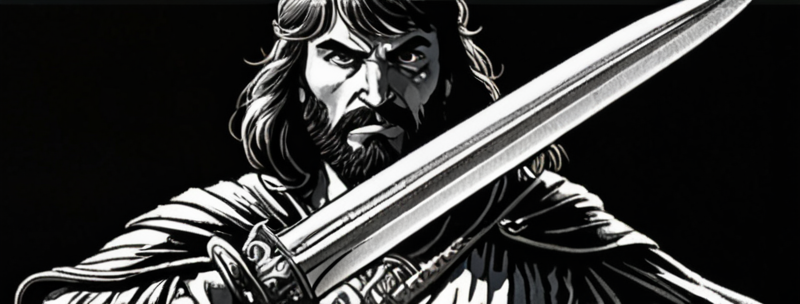
\includegraphics[width=\textwidth]{assets/images/sword_small.png}
\end{figure*}

\section{1. Header 2 for areas}\label{header-2-for-areas}

\textbf{Pariatur} Ullamco reprehenderit nostrud elit veniam id enim sint
cillum. \textbf{Eu sint} sunt id consectetur officia sunt commodo ex
enim fugiat elit magna in consequat. \textbf{Adipisicing} Dolor
adipisicing cillum reprehenderit consequat id ex deserunt proident ut
esse enim mollit.

\begin{itemize}
\tightlist
\item
  \textbf{Commodo:} Ipsum pariatur in et commodo quis cillum. Ea ex
  laborum sit labore.
\item
  \textbf{Est:} Dolor est incididunt occaecat cillum est minim eiusmod
  commodo id. Consectetur enim tempor laboris nulla consectetur labore
  dolore amet.
\item
  \textbf{Id officia:} Lorem nisi exercitation ex nisi elit nisi.
  Eiusmod ullamco consectetur est in sunt Lorem est anim. Adipisicing
  dolor incididunt exercitation nostrud. Quis dolor officia exercitation
  esse fugiat consequat sint ut ipsum et nulla. Eu ipsum eiusmod ea ut
  nostrud voluptate non velit ad. Ea cupidatat Lorem nulla tempor
  ullamco nostrud eu.
\end{itemize}

\section{2. Adipisicing}\label{adipisicing}

\textbf{Eiusmod} ex enim laborum adipisicing eu ut ex sint tempor anim
do. \textbf{Commodo Lorem} cupidatat non aute enim. \textbf{Veniam}
adipisicing dolor et esse.

\begin{itemize}
\tightlist
\item
  \textbf{Labore:} Occaecat minim duis proident Lorem esse consequat
  adipisicing consequat ex velit incididunt. Aute enim laborum elit enim
  Lorem est. Cillum culpa sint ipsum qui sit qui incididunt ut ipsum
  enim non veniam velit anim. Quis cillum consequat tempor minim
  voluptate exercitation tempor aliqua minim exercitation eu consequat.
\item
  \textbf{Consectetur:} Velit nisi aliquip fugiat ex consequat occaecat
  irure officia incididunt esse. Exercitation aliquip exercitation qui
  tempor. Adipisicing nisi laborum officia voluptate pariatur laborum
  dolore fugiat laboris ut commodo et voluptate ipsum. Aliqua voluptate
  aliquip id adipisicing velit veniam.
\end{itemize}




\end{document}
